\documentclass[10pt]{article}
\usepackage{../../local}
\urlstyle{same}

\newcommand{\classcode}{Physics C191}
\newcommand{\classname}{Introduction to Quantum Computing}
\renewcommand{\maketitle}{%
\hrule height4pt
\large{Eric Du \hfill \classcode}
\newline
\large{HW 05} \Large{\hfill \classname \hfill} \large{\today}
\hrule height4pt \vskip .7em
\small{Header styling inspired by CS 70: \url{https://www.eecs70.org/}}
\normalsize
}
\linespread{1.1}
\begin{document}
	\maketitle
	\section*{Collaborators}
	I worked closely with \textbf{Teja Nivarthi} on this assignment. 
	\section*{Problem 1}
	Alice has a pair of qubits \( a_1, a_2 \) which have been prepared in the Bell state
	\( \ket*{\Phi^{+}} = \frac{1}{\sqrt{2} }(\ket*{00} + \ket*{11}) \) 

	Alie would like to teleport this entangled state to Bob and Charlie such that they will share an entangled
	state \( \ket*{\Phi^{+}} \) between their respective qubits. 

	She follows the standard quantum teleportation protocol. A source sends an entangled qubit pair \( b_1, b_2 \) 
	to Alice and Bob, respectively, and also sends an entangled qubit pair \( c_1, c_2 \) to Alice and 
	Charlie, respectively. Each qubit pair is in the Bell state \( \ket*{\Phi^{+}} \). The following eleportation 
	scheme is then executed (note that this is the same scheme that was presented in lecture, only now 
	we are applying it twice because alice wants to teleport two qubits):
	%diagram
	(Diagram clarifications: The measuremet icon refers to a standard basis measurement. The standard notation 
	for CNOT is used here, where the filled in circle \( \bullet \) is the control qubit and the open circle
	\( \oplus \) is the target qubit.)

	Since each of the three pairs of qubits is initially in the state \( \ket*{\Phi^{+}} \), the initial 
	six-qubit state can be written as:
	\begin{multline*}
	\ket*{\Phi^{+}}\ket*{\Phi^{+}}\ket*{\Phi^{+}} = \frac{1}{\sqrt{2} }(\ket*{00}+ \ket*{11}) 
	\frac{1}{\sqrt{2} }(\ket*{00} + \ket*{11}) \frac{1}{\sqrt{2} }(\ket*{00} + \ket*{11}) \\
	= \frac{1}{2\sqrt{2}  }(\ket*{000000} + \ket*{000011} + \ket*{001100} + \ket*{001111} + 
	\ket*{110000} + \ket*{110011} + \ket*{111100} + \ket*{111111})
	\end{multline*} 
	where the qubit ordering we have used in writing out these states is \( \ket*{a_1a_2b_1b_2c_1c_2} \). 

	\begin{enumerate}[label=\alph*)]
		\item What is the state of the system after both CNOT gates have been executed? 

			\begin{solution}
				The CNOT gate applies to bits \( a_1, b_1  \) and \( a_2, c_1 \), so therefore the state looks like:
				\[
					\ket*{\psi} = \frac{1}{2\sqrt{2} }(\ket*{000000} + \ket*{000011} + \ket*{001100} + \ket*{001111}
					+ \ket*{111010} + \ket*{111001} + \ket*{110110} + \ket*{110101})
				\]
			\end{solution}
		\item What is the state of the system after both Hadamard gates have been executed? 

			\begin{solution}
				Now we need to apply the Hadamard gates. Recall that a hadamard gate turns the states:
				\[
				\ket*{0} \to \frac{\ket*{0} + \ket*{1}}{\sqrt{2} } \quad 
				\ket*{1} \to \frac{\ket*{0} - \ket*{1}}{\sqrt{2} }
				\] 
				Now, we'll be applying the Hadamard gate to \( a_1 \) and \( a_2 \), so therefore:
				\begin{multline*}
				\ket*{\psi} = \frac{1}{4\sqrt{2} }\biggr[\left( \frac{\ket*{0} + \ket*{1}}{\sqrt{2} } \right)^2
					(\ket*{0000} + 
				\ket*{0011} + \ket*{1100} + \ket*{1111})\\ + \left( \frac{\ket*{0} - \ket*{1}}{\sqrt{2} } \right)^2
			(\ket*{1010} + \ket*{1001} + \ket*{0110} + \ket*{0101})\biggr]
			\end{multline*} 
			I refuse to write down all 32 possible states.  
			\end{solution}
		\item Now assume that the measurements all contain a result of 0, such that the \( X \) and \( Z \) gates
			 are not executed. What is the final state of the system? Was alice successful in teleporting the 
			 entangled state to Bob and Charlie?

			 \begin{solution}
			 	If both measurements return zero, the final state of the system is acutally very simple, and consists 
				only of two terms, since the measurements ensure that \( a_1, a_2, b_1, c_1 \) are all zero. Therefore, 
				this corresponds to the states:
				\[
				\ket*{\psi} = \frac{1}{\sqrt{2} }(\ket*{000000} + \ket*{000101}) = \frac{1}{\sqrt{2} }\ket*{00}
				(\ket*{0000} + \ket*{0101})
				\] 
				This final state is precisely the entangled state we wanted (\( b_2 \) and \( c_2 \) ) are entangled
				with each other, so Alice was indeed successful in this case.
			 \end{solution}
	\end{enumerate}
	\pagebreak
	\section*{Problem 2}
	In this question, we will show the following fact about the quantum Fourier transform applied to quantum states 
	with periodic amplitudes:

	Suppose that you have a quantum state 
	\[
	\ket*{\psi} = \sum_{k=1}^{N-1} \alpha_k \ket*{k}
	\] 
	with periodic amplitudes (\( \alpha_k = \alpha_{k + t} \) mod \( N \) for some \( 1 \le t \le N-1 \)). Note that 
	periodicity requires that \( t \) divides \( N \). 

	We will show that 
	\[
	\text{QFT}_N\ket*{\psi} = \sum_{k=1}^{N-1} \beta_k \ket*{k}
	\] 
	where \( \beta_k \neq 0  \) only if \( k \) is an integer multiple of \( N/t \).
	\begin{enumerate}[label=\alph*)]
		\item Show that if \( \ket*{\psi} \)'s amplitudes are periodic with period \( t \) (i.e., 
			\( \alpha_k = \alpha_{k + t \text{ mod } N} \)), then it is equivalent to the state 
			\( \ket*{\psi + t } \):
			\[
			\ket*{\psi + t} = \sum_{k=1}^{N-1} \alpha_k \ket*{k + t \ \text{mod }N}
			\] 

			\begin{solution}
				Since we know that \( \alpha_k = \alpha_{k + t \text{ mod } N} \), then we know that the coefficient 
				attached to \( \ket*{k + t \text{ mod } N}  \) is the same as \( \alpha_k \). Thus, for all 
				states \( \ket*{k + t \text{ mod } N} \), they all share the same \( \alpha_k \). 
			\end{solution}
		\item Recall that the \( N' \)-th root of unity \( \omega_N = e^{i \frac{2\pi}{N}}\). Show that 
			\( \omega_N^{r} = 1 \) if and only if \( r \) is an integer multiple of \( N \). 

			\begin{solution}
				We show first that \( \omega_N^{r} = 1 \) if \( r  \) is a multiple of \( N \).  This means we can 
				write \( r = kN \) for some \( k \), and therefore:
				\[
				\omega_N^{r} = e^{i \frac{2\pi}{N} \cdot kN} = e^{i 2 \pi k}
				\] 
				And since \( k \) is an integer, then we know that \( \omega_N^{r} = 1 \). For the reverse side, 
				we we know  \( \omega_N^{r} \) can be written as:
				\[
				\omega_N ^{r} = e^{i \frac{2\pi}{N} r}
				\] 
				If this must equal 1, then it must be the case that \( i \frac{2\pi}{N} r = k (2\pi i) \), 
				which implies that \( r \) must be a multiple of \( N \). 
			\end{solution}
		\item Using that the quantum Fourier transforms of \( \ket*{\psi} \) and \( \ket*{\psi + t} \) are 
			related in the following way. If 
			\[
			\text{QFT}_N \ket*{\psi} = \sum_{k=1}^{N-1} \beta_k \ket*{k}
			\] 
			then 
			\[
			\text{QFT}_N \ket*{\psi + t} = \sum_{k=1}^{N-1} \omega_N^{kt}\beta_k \ket*{k}
			\] 
			Show that if \( \ket*{\psi} = \ket*{\psi + t} \), then \( \text{QFT}_N\ket*{\psi} \) has nonzero 
			amplitudes only on integer multiples of \( N / t \). That is, show that if \( \beta_k \neq 0 \), 
			then \( k = \ell (N / t) \) for some integer \( \ell \). 

			\begin{solution}
				If \( \ket*{\psi} = \ket*{\psi + t}\), then we also know that applying \( \text{QFT}_N \) on both 
				states should return the same values. Therefore, we have:
				\[
				\sum_{k=1}^{N-1} \beta_k \ket*{k} = \sum_{k=1}^{N-1} \omega_N^{kt}\beta_k \ket*{k}
				\] 
				If \( \beta_k \neq 0 \), then we have:
				\[
				\omega_N ^{kt} = 1
				\] 
				Then from part (b), we know that this implies that \( kt \) must be a multiple of \( N \), and one 
				way to guarantee that is to let \( k = \ell(N / t) \) for some integer  \( \ell \), as desired. 
			\end{solution}
	\end{enumerate}
	\pagebreak
	\section*{Problem 3}
	In this question, we will go through a small example of Schor's factoring algoritihm. Use the following facts about 
	the quantum Fourier transform (\( \text{QFT}_M \)) applies to periodic and shifted states:
	\begin{enumerate}[label=\arabic*)]
		\item QFT on periodic states: Let \( 1 < r < M \) be an integer that divides \( M \). \( \text{QFT}_M \) 
			applied to the state \( \sqrt{\frac{r}{M}} (\ket*{0} + \ket*{r} + \ket*{2r} + \cdots + \ket*{M - r})\)
			results in 
			\[
			\frac{1}{\sqrt{r} }(\ket*{0 } + \ket*{M / r} + \ket*{2 M / r} + \cdots + \ket*{(r - 1) M /r})
			\] 
		\item QFT on shifted states: If \( \ket*{\psi} = \sum_{k=0}^{M-1} \alpha_k \ket*{k} \) and 
			\( \ket*{\psi + t} = \sum_{k=0}^{M-1} \alpha_k \ket*{k + t \ \text{mod } N} \), then \( \text{QFT}_M \) 
			applied to the two states are related by: If 
			\[
			\text{QFT}_M \ket*{\psi} = \sum_{k=0}^{M-1} \beta_k \ket*{k}
			\] 
			then 
			\[
			\text{QFT}_M \ket*{\psi + t} \sum_{k=0}^{M-1} \omega_M^{kt}\beta_k \ket*{k}
			\] 
			We will work through an example of factoring \( N = 21 \) using \( \text{QFT}_M \) with \( M = 12 \). 
	\end{enumerate}
	\begin{enumerate}[label=\alph*)]
		\item Let \( a = 2 \). Calculate the state \( \ket*{\psi} = \sum_{x=0}^{M-1} \ket*{x} \ket*{a^{x} \ 
			\text{mod } N} \). 

			\begin{solution}
				Written out, since \( M = 12 \), and \( N = 21 \), this state is equal to:
				\[
					\ket*{\psi} = \ket*{0}\ket*{1} + \ket*{1}\ket*{2} + \ket*{2}\ket*{4} + \cdots + 
					\ket*{10}\ket*{16} + \ket*{11}\ket*{11}
				\] 
				The higher powers of 2 were computed using Mathematica. 
			\end{solution}
		\item Suppose we measure the second register of \( \ket*{\psi} \) and obtain "1". 
			What is the resulting state on the first register, then perform \( \text{QFT}_M \) on the first 
			register. What is the resulting state on the first register? Now measure this state in the standard 
			basis. What are the possible measurement outcomes? 

			\begin{solution}
				If we obtain 2 in the second register, then the state after this measurement corresponds to the states 
				\( \ket*{x} \) where \( 2^{x} \equiv 1 \pmod N \). It turns out that this refers to every multiple 
				of \( 6 \), so therefore the state for the first register is now:
				\[
				\ket*{\psi'} = \frac{1}{2}(\ket*{0} + \ket*{6} + \ket*{12} + \ket*{18})
				\] 
				Then, performing \( QFT_M \) on this, we use rule 1: 
				\[
				\text{QFT}_M\ket*{\psi'} = \frac{1}{\sqrt{6} }(\ket*{0} + \ket*{21 / 6} + \ket*{42/6} + 
				\ket*{63 / 6} + \ket*{84 / 6})
				\] 
			\end{solution}
		\item Suppose we repeat the above experiment, now the first step (when measuring the second register) gives "4".
			Answer the same questions as above. 

			\begin{solution}
				Repeating what was done above, the state is now:
				\[
				\ket*{\psi'} = (\ket*{2} + \ket*{8} + \ket*{14} + \ket*{20})
				\] 
			\end{solution}
		\item Suppose we repeat the above experiment 4 times in total. Each time we record a measurement outcome of
			the first register (after performing \( \text{QFT}_M \) ). Suppose the recorded outcomes are all different.
			What is their greatest common divisor \( g \)?
		\item Calculate \( \mathrm{gcd}(N, a^{M / 2g} - 1) \) and \( \mathrm{gcd}(N, a^{M / 2g} + 1) \). Are they 
			prime factors of \( N \)? 
	\end{enumerate}
	\pagebreak
	\section*{Problem 4}
	In this question, we'll try to get a geometric understanding of Grover's algorithm. In Grover's algorithm 
	we have some distinguished, marked element \( a \in \{1, \dots, N\} = [N] \) and have access to some function 
	\( f: [N] \to \{0, 1\}  \) that recognized a, i.e., \( f(a) = 1 \) and \( f(x) = 0 \) if \( x \neq a \). 
	Our goal is to use \( f \) to find \( a \). 

	Let \( \ket*{a} \) be the standard basis state labelled with \( a\) and define
	\[
		\ket*{e} = \frac{1}{\sqrt{N - 1} }\sum_{\text{\( x \in [N] \) and \( x \neq a \)}} \ket*{x}
	\] 
	At all times, we will maintain a quanutm state in the two-dimensinoal subspace spanned by \( \ket*{a} \) and 
	\( \ket*{e} \). That is, our state can be written as 
	\( \alpha \ket*{a} + \beta\ket*{e} i\ (\alpha, \beta \in \R)\) and therefore we can understand the algorithm 
	in a two dimensional space.
	\begin{enumerate}[label=\alph*)]
		\item We start with the state \( \ket*{u} = \frac{1}{\sqrt{N} }\sum_{x \in [N]}\ket*{x} \). Express 
			\( \ket*{u} \) in terms of \( \ket*{a} \) and \( \ket*{e} \). What is the angle \( \theta \) between 
			\( \ket*{u} \) and \( \ket*{e} \) in the following two dimensional space? 
			% diagram

			\begin{solution}
				We have the state \( \ket*{u} \), which we can write as: 
				\[
				\ket*{u} = \frac{1}{\sqrt{N} }(\ket*{a} + \ket*{e}) = \frac{1}{\sqrt{N} }\ket*{a} + 
				\sqrt{\frac{N-1}{N}} \ket*{e}
				\] 
				Now, the angle between \( \ket*{u} \) and \( \ket*{e} \) is given by the equation:
				\[
				\sin \theta = \frac{1}{\sqrt{N} } \implies \theta = \sin^{-1}\left( \frac{1}{\sqrt{N} } \right) 
				\] 
			\end{solution}
		\item Apply the oracle \( U_f \) (defined as \( U_f \ket*{x} = (-1)^{f(x)}\ket*{x} \) ) to 
			\( \ket*{u} \), obtaining the state \( \ket*{\psi} \). Draw \( \ket*{\psi} \) in the above two 
			dimensional space.

			\begin{solution}
				We do as instructed, and compute \( U_f \ket*{u} \):
				\begin{align*}
					U_f\ket*{u} &= \frac{1}{\sqrt{N} }(-1)^{f(a)}\ket*{a} + \sqrt{\frac{N-1}{N}} 
					\sum_{x \neq a} (-1)^{f(x)} \ket*{x}\\
				\end{align*}
				Then, since we have that \( f(a) = 1 \) and 0 for all other values everything in the state 
				\( \ket*{e} \) 
				will evaluate to 1, and hence that part will remain unchanged. Therefore, we have:
				\[
				U_f \ket*{u} = -\frac{1}{\sqrt{N} }\ket*{a} + \sqrt{\frac{N-1}{N}} \ket*{e}
				\] 
				The state in the diagram would look like:
				\begin{center}
					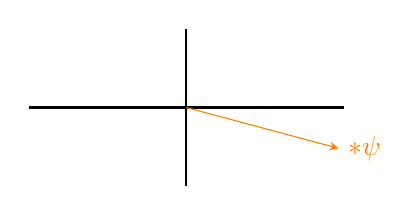
\begin{tikzpicture}
						\draw[thick] (-2, 0) --(2, 0);
						\draw[thick] (0, -1) -- (0, 1);
						\draw[-stealth, orange] (0, 0) -- (-15:2) node[right] {\( \ket*{\psi} \) };
					\end{tikzpicture}
				\end{center}
			\end{solution}
		\item Apply the unitary \( 2\ket*{u}\bra*{u} - I \) to the state \( \ket*{\psi} \). Draw the resulting 
			state in the above two dimensional space. 

			\begin{solution}
				We are asked to compute \( (2 \ket*{u}\bra*{u} - I) \ket*{\psi} \). To do this, it's benefiical 
				to rewirte \( \ket*{\psi} \) in terms of \( u \), so that the outer product may be applied nicely. 
				Rearranging:
				\[
				\ket*{\psi} = -\frac{1}{\sqrt{N} }\ket*{a} + \sqrt{\frac{N-1}{N}} \ket*{e}
				= \ket*{u} - \frac{2}{\sqrt{N} }\ket*{a}
				\] 
				Therefore, now applying the unitary:
				\begin{align*}
					\ket*{\psi'} = 
					(2 \ket*{u}\bra*{u} - I) \ket*{\psi} &= (2\ket*{u}\bra*{u} - I)\ket*{u} - \frac{2}{\sqrt{N} }
					(2\ket*{u}\bra*{u} - I)\ket*{a}\\
					&= \ket*{u} - \frac{2}{\sqrt{N} }\left(\frac{2}{\sqrt{N} }\ket*{u} - \ket*{a}\right)\\
					&= \left(1-\frac{4}{N}\right)\ket*{u} + \frac{2}{\sqrt{N} }\ket*{a} 
				\end{align*}
			\end{solution}
		\item Apply the operation \( (2\ket*{u}\bra*{u} - I) U_f \) two more times on the resulting state 
			from 2.3 and draw the two resulting states in the above two dimensinoal space. What angle of rotation does 
			\( (2\ket*{u}\bra*{u} - I)U_f \) perform in the space? 

			\begin{solution}
				To preface, there's a lot of algebra that I'll skip in this problem, but it's basically the same thing 
				we did in part (c) except twice. Applying the unitary to \( \ket*{\psi'} \):
				\begin{align*}
					\ket*{\psi''} = (2\ket*{u}\bra*{u} - I) \ket*{\psi'} &= 
					(2 \ket*{u}\bra*{u} - I) \left( 1 - \frac{4}{N} \right) 
					\ket*{u} - \frac{2}{\sqrt{N} }(2 \ket*{u}\bra*{u} - I) \ket*{a}\\
					&= \left( 1 - \frac{4}{N} \right) \ket*{u} - \frac{4}{N}\ket*{u} + \frac{2}{N}\ket*{a}\\
					&= \left( 1- \frac{8}{N} \right) \ket*{u} + \frac{2}{\sqrt{N}}\ket*{a} 
				\end{align*} 
				By this point we can start to notice a pattern: all this operator does is add another \( -\frac{4}{N}
				\ket*{u}\) to the state, so therefore we can extrapolate:
				\[
				\ket*{\psi'''} = (2\ket*{u}\bra*{u} - I) \ket*{\psi''} = \ket*{\psi''} - \frac{4}{N}\ket*{u}
				= \left( 1 - \frac{12}{N} \right) \ket*{u} + \frac{2}{\sqrt{N} }\ket*{a}
				\] 
				Re-expressing this in terms of \( \ket*{a} \) and \( \ket*{e} \):
				\[
				\ket*{\psi'''} = \sqrt{\frac{N}{N-1}} \left( 1 - \frac{12}{N} \right) \ket*{e} + \frac{1}{\sqrt{N} }
				\left(3 - \frac{12}{N}\right)\ket*{a}
				\] 
				So now our new angle is:
				\[
				\theta = \sin^{-1}\left( \frac{3}{\sqrt{N} }\left( 1 - \frac{4}{N} \right)  \right) 
				\] 
				In general, we can see that applying this operator rotates our state counterclockwise by \( 2\theta_0 \)
				every time, where \( \theta_0 \) is the initial angle we started with (in \( \ket*{\psi} \)). 
			\end{solution}
		\item Grover's algorithm repeatedly applies \( (2 \ket*{u} \bra*{u} - I) U_f \) to \( \ket*{u} \) to get 
			close to \( \ket*{a} \). How many times should you apply this operation to et 
			closest to the state \( \ket*{a} \)? (You can use the small angle approximation
			\( \sin \theta \approx \theta \)).

			\begin{solution}
				In order for us to get closest to \( \ket*{a} \), then the requirement is that we want to get 
				an angle as close to \( \frac{\pi}{2} \) as possible. From the previous part, we can deduce that
				after applying the operator \( k \) times, we have a total angle of \( \theta = (2k + 1)\theta_0 \), 
				meaning that we have to solve the equation:
				\[
					(2k+1)\sin^{-1}\left( \frac{1}{\sqrt{N} } \right)  = \frac{\pi}{2}
				\] 
				Using the small angle approximation (valid when \( N \) large), we can get rid of the sine, and 
				also get rid of the 1 in from of \( 2k + 1 \), since when \( N \) is large we also implicitly assume 
				that the initial angle is very close to zero. This means that:
				\[
				k \approx \frac{\pi \sqrt{N} }{4}
				\] 
			\end{solution}
	\end{enumerate}
\end{document}
